% UltraLight VM-UNet -- architecture diagram.
%
% Mirrors UltraLight_VM_UNet.forward() in models/UltraLight_VM_UNet.py exactly:
% channel counts, spatial resolutions, and which skip tensor (t1..t5) is added
% at which decoder stage. Node "level" (its row) is its OUTPUT resolution --
% e.g. encoder1 outputs t1 at 128^2, so it sits on the 128^2 row; decoder5's
% output (after its own upsample) is also 128^2, and is where t1 gets added,
% so decoder5 sits on the same row. That row-per-resolution scheme is what
% makes every skip connection below a plain horizontal line.
%
% encoder6 (the bottleneck) and decoder1 are BOTH at 8^2 -- encoder6 has no
% downsample of its own, and decoder1 has no upsample of its own -- so they
% flank the bottom of the U rather than sitting on a shared row with encoder5.
%
% Compile: pdflatex architecture.tex  ->  architecture.pdf (tightly cropped)

\documentclass[tikz,border=10pt]{standalone}
\usepackage{amsmath}
\usetikzlibrary{arrows.meta,positioning}

\begin{document}
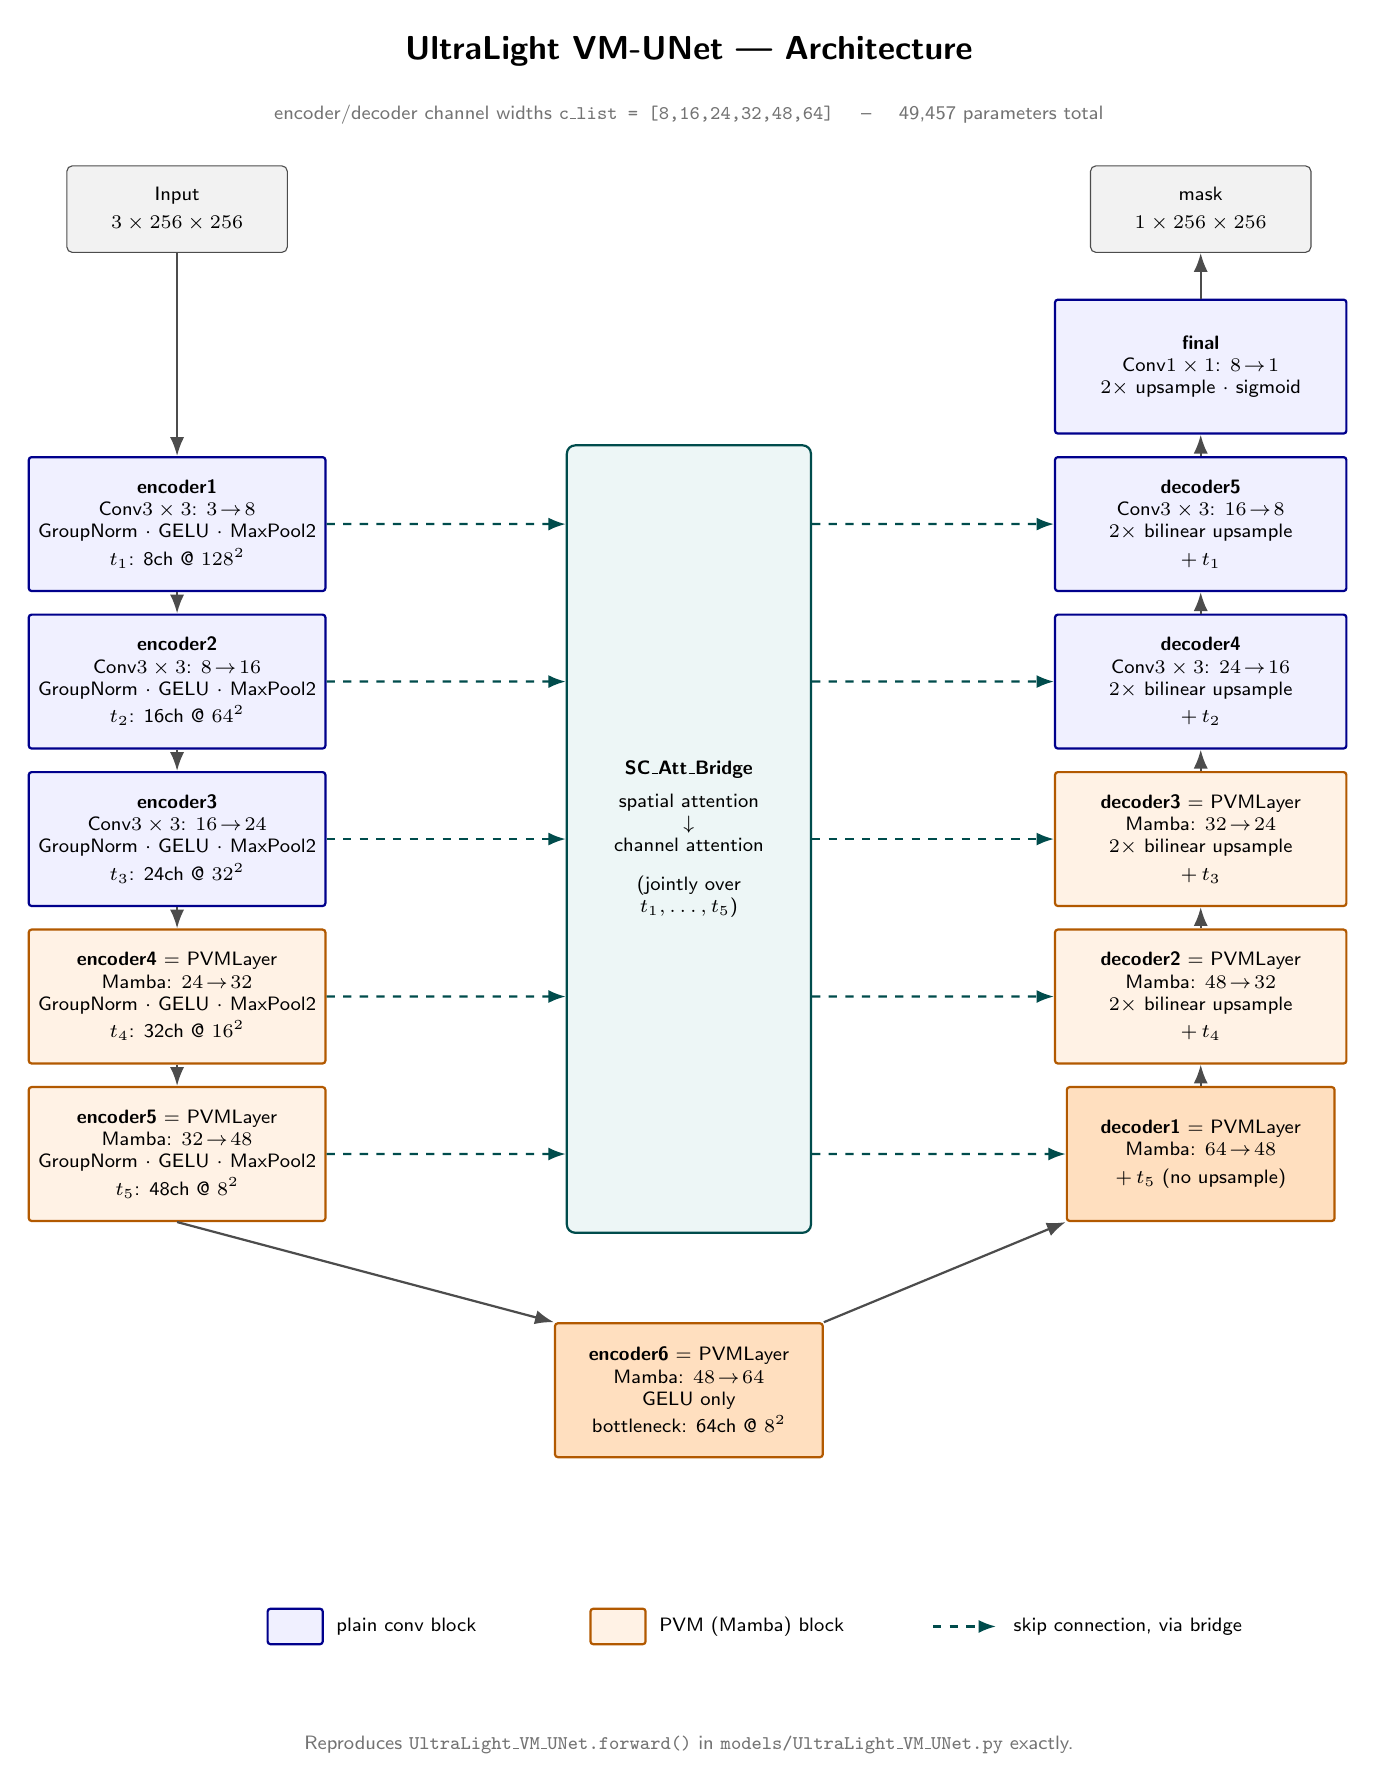
\begin{tikzpicture}[
  >=Latex,
  every node/.style={font=\sffamily},
  io/.style={rectangle, rounded corners=2pt, draw=black!70, fill=black!5,
             minimum width=2.8cm, minimum height=1.1cm, align=center,
             font=\sffamily\scriptsize},
  conv/.style={rectangle, rounded corners=1pt, draw=blue!55!black, fill=blue!6,
               thick, minimum width=3.7cm, minimum height=1.7cm, align=center,
               font=\sffamily\scriptsize},
  pvm/.style={rectangle, rounded corners=1pt, draw=orange!70!black, fill=orange!10,
              thick, minimum width=3.7cm, minimum height=1.7cm, align=center,
              font=\sffamily\scriptsize},
  bottleneck/.style={rectangle, rounded corners=1pt, draw=orange!70!black, fill=orange!25,
              thick, minimum width=3.4cm, minimum height=1.7cm, align=center,
              font=\sffamily\scriptsize},
  bridgebox/.style={rectangle, rounded corners=3pt, draw=teal!60!black, fill=teal!7,
              thick, minimum width=3.1cm, minimum height=10cm, align=center,
              font=\sffamily\scriptsize, text width=2.6cm},
  flow/.style={-{Latex[length=2.4mm]}, thick, black!70},
  skip/.style={-{Latex[length=2.2mm]}, dashed, teal!60!black, thick},
]

% ---------------------------------------------------------------- title --
\node[font=\sffamily\bfseries\large] at (6.5,17) {UltraLight VM-UNet --- Architecture};
\node[font=\sffamily\scriptsize, text=black!55] at (6.5,16.2)
  {encoder/decoder channel widths \texttt{c\_list = [8,16,24,32,48,64]} \quad -- \quad 49{,}457 parameters total};

% -------------------------------------------------------------- encoder --
\node[io]  (input) at (0,15) {Input\\[2pt]$3\times256\times256$};
\node[conv] (e1) at (0,11) {\textbf{encoder1}\\Conv$3\times3$: $3\!\to\!8$\\GroupNorm $\cdot$ GELU $\cdot$ MaxPool2\\[2pt]$t_1$: 8ch @ $128^2$};
\node[conv] (e2) at (0,9)  {\textbf{encoder2}\\Conv$3\times3$: $8\!\to\!16$\\GroupNorm $\cdot$ GELU $\cdot$ MaxPool2\\[2pt]$t_2$: 16ch @ $64^2$};
\node[conv] (e3) at (0,7)  {\textbf{encoder3}\\Conv$3\times3$: $16\!\to\!24$\\GroupNorm $\cdot$ GELU $\cdot$ MaxPool2\\[2pt]$t_3$: 24ch @ $32^2$};
\node[pvm]  (e4) at (0,5)  {\textbf{encoder4} = PVMLayer\\Mamba: $24\!\to\!32$\\GroupNorm $\cdot$ GELU $\cdot$ MaxPool2\\[2pt]$t_4$: 32ch @ $16^2$};
\node[pvm]  (e5) at (0,3)  {\textbf{encoder5} = PVMLayer\\Mamba: $32\!\to\!48$\\GroupNorm $\cdot$ GELU $\cdot$ MaxPool2\\[2pt]$t_5$: 48ch @ $8^2$};
\node[bottleneck] (e6) at (6.5,0) {\textbf{encoder6} = PVMLayer\\Mamba: $48\!\to\!64$\\GELU only\\[2pt]bottleneck: 64ch @ $8^2$};

% -------------------------------------------------------------- decoder --
\node[bottleneck] (d1) at (13,3) {\textbf{decoder1} = PVMLayer\\Mamba: $64\!\to\!48$\\[2pt]$+\,t_5$ (no upsample)};
\node[pvm]  (d2) at (13,5)  {\textbf{decoder2} = PVMLayer\\Mamba: $48\!\to\!32$\\$2\times$ bilinear upsample\\[2pt]$+\,t_4$};
\node[pvm]  (d3) at (13,7)  {\textbf{decoder3} = PVMLayer\\Mamba: $32\!\to\!24$\\$2\times$ bilinear upsample\\[2pt]$+\,t_3$};
\node[conv] (d4) at (13,9)  {\textbf{decoder4}\\Conv$3\times3$: $24\!\to\!16$\\$2\times$ bilinear upsample\\[2pt]$+\,t_2$};
\node[conv] (d5) at (13,11) {\textbf{decoder5}\\Conv$3\times3$: $16\!\to\!8$\\$2\times$ bilinear upsample\\[2pt]$+\,t_1$};
\node[conv] (final) at (13,13) {\textbf{final}\\Conv$1\times1$: $8\!\to\!1$\\$2\times$ upsample $\cdot$ sigmoid};
\node[io]   (output) at (13,15) {mask\\[2pt]$1\times256\times256$};

% ---------------------------------------------------------------- bridge --
\node[bridgebox] (bridge) at (6.5,7)
  {\textbf{SC\_Att\_Bridge}\\[4pt]spatial attention\\$\downarrow$\\channel attention\\[6pt](jointly over\\$t_1,\dots,t_5$)};

% ----------------------------------------------------------- main flow --
\draw[flow] (input.south) -- (e1.north);
\draw[flow] (e1.south) -- (e2.north);
\draw[flow] (e2.south) -- (e3.north);
\draw[flow] (e3.south) -- (e4.north);
\draw[flow] (e4.south) -- (e5.north);
\draw[flow] (e5.south) -- (e6.north west);
\draw[flow] (e6.north east) -- (d1.south west);
\draw[flow] (d1.north) -- (d2.south);
\draw[flow] (d2.north) -- (d3.south);
\draw[flow] (d3.north) -- (d4.south);
\draw[flow] (d4.north) -- (d5.south);
\draw[flow] (d5.north) -- (final.south);
\draw[flow] (final.north) -- (output.south);

% ------------------------------------------------- skip connections (t1..t5) --
\draw[skip] (e1.east) -- ([yshift=4cm]bridge.west);
\draw[skip] ([yshift=4cm]bridge.east) -- (d5.west);
\draw[skip] (e2.east) -- ([yshift=2cm]bridge.west);
\draw[skip] ([yshift=2cm]bridge.east) -- (d4.west);
\draw[skip] (e3.east) -- (bridge.west);
\draw[skip] (bridge.east) -- (d3.west);
\draw[skip] (e4.east) -- ([yshift=-2cm]bridge.west);
\draw[skip] ([yshift=-2cm]bridge.east) -- (d2.west);
\draw[skip] (e5.east) -- ([yshift=-4cm]bridge.west);
\draw[skip] ([yshift=-4cm]bridge.east) -- (d1.west);

% --------------------------------------------------------------- legend --
\node[conv, minimum width=0.7cm, minimum height=0.45cm] (leg1) at (1.5,-3) {};
\node[anchor=west, font=\sffamily\scriptsize] at (1.9,-3) {plain conv block};
\node[pvm, minimum width=0.7cm, minimum height=0.45cm] (leg2) at (5.6,-3) {};
\node[anchor=west, font=\sffamily\scriptsize] at (6.0,-3) {PVM (Mamba) block};
\draw[skip] (9.6,-3) -- (10.4,-3);
\node[anchor=west, font=\sffamily\scriptsize] at (10.5,-3) {skip connection, via bridge};

\node[font=\sffamily\scriptsize, text=black!55] at (6.5,-4.5)
  {Reproduces \texttt{UltraLight\_VM\_UNet.forward()} in \texttt{models/UltraLight\_VM\_UNet.py} exactly.};

\end{tikzpicture}
\end{document}
